\chapter{Sistema implementato}
\section{Panoramica ad alto livello}
Il sistema che abbiamo implementato \`e una \emph{web-app} la cui funzione \`e quella di ricercare il cammino minimo in un grafo con topologia a griglia, dati due particolari nodi: uno di partenza e uno di arrivo.\\*
Una \emph{griglia} \`e rappresentata attraverso una matrice $A \in \mathbb{N}^{n x n}$ siffatta:
\[ A=[a_{i,j}] \]
Dove $a_{i,j}>0 \iff \exists $ un nodo nella riga i e colonna j della griglia rappresentata da $A$ e $n$ \`e il numero massimo di righe e colonne ammesso per la griglia che A rappresenta.\\*
Occorre precisare che in questa particolare topologia di grafo, ogni nodo $i,j$ pu\`o avere al pi\`u 4 vicini:
\begin{itemize}
	\item $i+1,j$
	\item $i-1,j$
	\item $i,j+1$
	\item $i,j-1$
\end{itemize} 
Pertanto il cammino minimo potr\`a attraversare archi solo in direzione orizzontale o verticale.\newpage
A titolo di esempio, si consideri la matrice in tabella 1.
\begin{table}[]
	\centering
	\caption{Matrice A}
	\label{my-label}
	\begin{tabular}{|l|l|l|l|l|}
		\hline
		1 & 0 & 1 & 0 & 0 \\ \hline
		1 & 1 & 1 & 0 & 0 \\ \hline
		1 & 0 & 0 & 0 & 1 \\ \hline
		1 & 1 & 1 & 1 & 1 \\ \hline
		0 & 0 & 0 & 0 & 1 \\ \hline
	\end{tabular}
\end{table}
Supponiamo di voler cercare il camminimo minimo che parta dal nodo $0,0$ e che termini al nodo $4,4$ (nella fattispecie, esso \`e unico).
Si ottiene il risultato esposto in tabella 2.
\begin{table}[]
	\centering
	\caption{Cammino minimo relativo ad A}
	\label{my-label}
	\begin{tabular}{|l|l|l|l|l|}
		\hline
		\cellcolor[HTML]{68CBD0}1 & 0 & 1 & 0 & 0                         \\ \hline
		\cellcolor[HTML]{68CBD0}1 & 1 & 1 & 0 & 0                         \\ \hline
		\cellcolor[HTML]{68CBD0}1 & 0 & 0 & 0 & 1                         \\ \hline
		\rowcolor[HTML]{68CBD0} 
		1                         & 1 & 1 & 1 & 1                         \\ \hline
		0                         & 0 & 0 & 0 & \cellcolor[HTML]{68CBD0}1 \\ \hline
	\end{tabular}
\end{table}
\newpage
L'implementazione del suddetto sistema si articola in due componenti:
\begin{enumerate}
	\item Server
	\item Client
\end{enumerate}
Il Server, realizzato attraverso l'utilizzo del framework \emph{Spring Boot}, gestisce un database MongoDB contenente le matrici che rappresentano particolari griglie.\\*
Il Server deve poter essere in grado di gestire tre tipi di richieste pervenibili attraverso la sua interfaccia \emph{REST}: recuperare tutte le griglie salvate nel database, recuperarne una in particolare, oppure trovare un eventuale cammino minimo in una particolare griglia.\\*
Per quanto riguarda le operazioni \emph{CRUD} sul database, queste sono realizzate mediante un \emph{Web Controller} protetto da username e password. Occorre infine precisare che il server non \`e consapevole di colloquiare con una particolare istanza di un client, ci\`o comporta che le richieste vengano ugualmente servite sia nel caso in cui il client sia un normale browser, oppure il Client java che abbiamo realizzato.\\*
Il Client da noi implementato \`e un' applicazione Java che utilizza la libreria \emph{Swing} per fornire all'utente un'interfaccia grafica \emph{user-friendly}. Il Client \'e capace di eseguire le tre possibili richieste \emph{HTTP} inoltrabili all'interfaccia \emph{REST} del Server.
\begin{figure}[th]
	\centering
	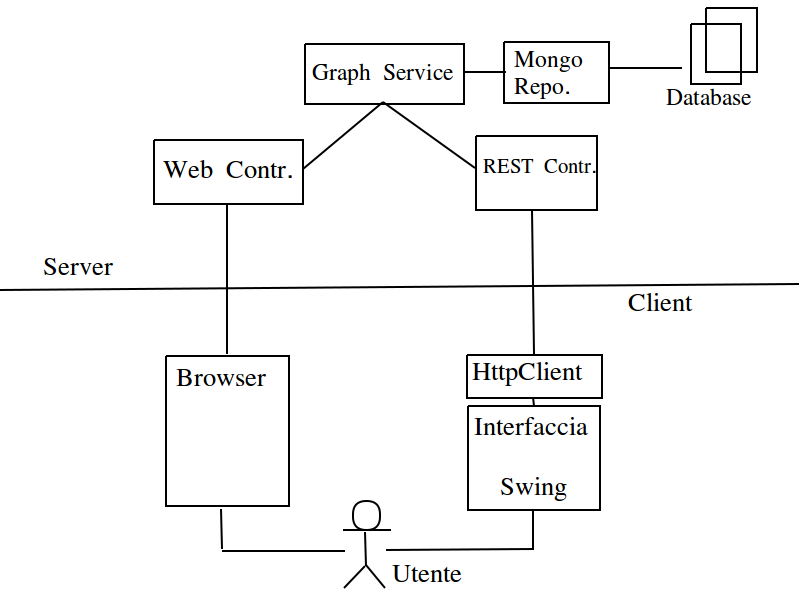
\includegraphics[width=0.7\linewidth]{Images/app-scheme}
	\caption[Schema UML-Like]{Schema che mostra il funzionamento del sistema implementato cos\`i come visto dall'utente}
	\label{fig:app-scheme}
\end{figure}

